\documentclass[12pt,spanish]{article}
\usepackage[spanish]{babel}
\usepackage{graphicx}
\usepackage{color}
\usepackage{xcolor}
\usepackage{colortbl}
\usepackage{amsthm,thmtools}
\usepackage{multirow}
\usepackage{amsmath}
\usepackage{subcaption}
\usepackage{adjustbox}
\usepackage{multirow}
\usepackage[hidelinks]{hyperref}
\usepackage{caption}
\usepackage{amsthm}
\usepackage{multicol}
\usepackage{float}
\usepackage{amsfonts}
\usepackage{titling}
\usepackage{soul}
\usepackage{listings}
\usepackage{mathtools}
\usepackage{array}
\usepackage{tikz}
\usepackage[framemethod=tikz]{mdframed}
\definecolor{light-gray}{gray}{0.95}

\graphicspath{ {../img/}}
\selectlanguage{spanish}
\usepackage[utf8]{inputenc}
\usepackage{graphicx}
\usepackage[a4paper,left=3cm,right=2cm,top=2.5cm,bottom=2.5cm]{geometry}

\newenvironment{solution}{
	\par
	\textbf{Solución}
	\par

}
{
}
\lstset{
  breaklines=true,
  postbreak=\mbox{\textcolor{red}{$\hookrightarrow$}\space},
}
\surroundwithmdframed[
  hidealllines=true,
  backgroundcolor=light-gray,
  innerleftmargin=0pt,
  innertopmargin=0pt,
  innerbottommargin=0pt]{lstlisting}


\title{Modelos de Computación}
\setlength{\droptitle}{10em}
\author{Carlos Sánchez Páez}

\makeindex
\begin{document}
\definecolor{light-gray}{gray}{0.95}
\lstset{columns=fullflexible,basicstyle=\ttfamily}
\surroundwithmdframed[
  hidealllines=true,
  backgroundcolor=light-gray,
  innerleftmargin=0pt,
  innertopmargin=0pt,
  innerbottommargin=0pt]{lstlisting}


\begin{titlepage}

 \newlength{\centeroffset}
 \setlength{\centeroffset}{-0.5\oddsidemargin}
 \addtolength{\centeroffset}{0.5\evensidemargin}
 \thispagestyle{empty}

 \noindent\hspace*{\centeroffset}
 \begin{minipage}{\textwidth}

  \centering
  
\includegraphics[width=0.9\textwidth]{logo_ugr.jpg}\\[1.4cm]

  \textsc{ \Large Modelos de Computación\\[0.2cm]}
  \textsc{GRADO EN INGENIERÍA INFORMÁTICA}\\[1cm]

  {\Huge\bfseries Prácticas resueltas\\}
 \end{minipage}

 \vspace{1.5cm}
 \noindent\hspace*{\centeroffset}
 \begin{minipage}{\textwidth}
  \centering

  \textbf{Autor}\\ {Carlos Sánchez Páez}\\[4ex]
  
\includegraphics[width=0.4\textwidth]{etsiit_logo.png}\\[0.1cm]
  \vspace{1.5cm}
  
\includegraphics[width=0.5\textwidth]{decsai.jpg}\\[0.1cm]
  \vspace{1cm}
  \textsc{Escuela Técnica Superior de Ingenierías Informática y de Telecomunicación}\\
  \vspace{1cm}
  \textsc{Curso 2019-2020}
 \end{minipage}
\end{titlepage}
\thispagestyle{empty}
\newpage
\tableofcontents{}
\newpage

\section{Práctica 1}

Construir un autómata finito determinístico para aceptar cadenas de ceros y unos que tengan un número de ceros que no sea múltiplo de 3. Usar JFLAP para simular el autómata.

\begin{solution}
	Para construir el siguiente autómata emplearemos la metodología inversa: elaboraremos uno que acepte un número de ceros múltiplo de 3 y cambiaremos sus estados finales por normales y viceversa, ya que así es más sencillo.\\
	Necesitaremos definir tres estados:
	\begin{itemize}
		\item $q_0$: hasta ahora el autómata ha leído un número de ceros múltiplo de 3. Es estado final y también inicial, ya que $\epsilon$, la cadena vacía, también debe ser aceptada (0 es múltiplo de 3).
		\item $q_1$: hemos leído un cero extra.
		\item $q_2$: hemos leído dos ceros extra.
	\end{itemize}
	Las transiciones serán las siguientes:
	\begin{itemize}
		\item Si leemos un uno, nos quedamos en el mismo estado: $q_0 \xRightarrow{1} q_0$, $q_1 \xRightarrow{1} q_1$ y $q_2 \xRightarrow{1} q_2$.
		\item Si leemos un cero, avanzamos al siguiente estado: $q_0 \xRightarrow{0} q_1$, $q_1 \xRightarrow{0} q_2$ y $q_2 \xRightarrow{0} q_0$.
	\end{itemize}
	Por tanto, nuestro autómata sería el siguiente:
	\begin{figure}[H]
		\centering
		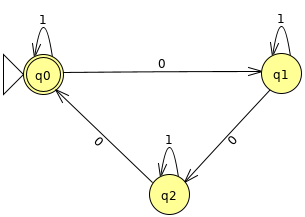
\includegraphics[width=0.5\textwidth]{p1-1.png}
	\end{figure}
	Ahora cambiamos los estados normales por finales y viceversa, obteniendo la solución al problema:
	\begin{figure}[H]
		\centering
		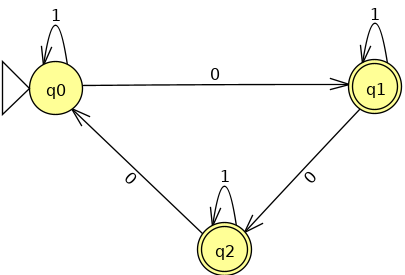
\includegraphics[width=0.5\textwidth]{p1-2.png}
	\end{figure}
\end{solution}
\newpage
\section{Práctica 2}
Plantear un lenguaje regular con un número infinito de cadenas. Obtener la expresión regular del lenguaje y convertirlo a AFD minimal y AFND con transiciones nulas mediante JFLAP.
\begin{solution}

Tomemos el siguiente lenguaje:
\[
		L = \{ ab^icd^je : i,j \in \mathbb{N}\}
\]
La expresión regular resultante es $ab^*cd^*e$. El AFND con transiciones nulas obtenido es el siguiente:
\begin{figure}[H]
	\centering
	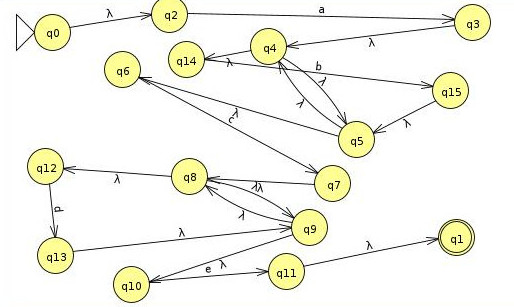
\includegraphics[width=0.5\textwidth]{p2-1.jpg}
\end{figure}

Lo convertimos a AFD y obtenemos:
\begin{figure}[H]
	\centering
	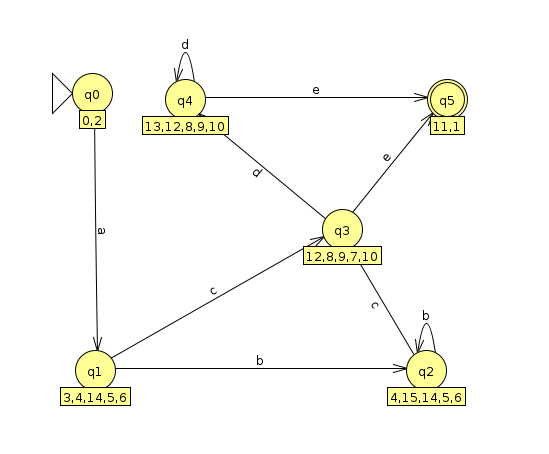
\includegraphics[width=0.5\textwidth]{p2-2.png}
\end{figure}

Finalmente, lo minimizamos:
\begin{figure}[H]
	\centering
	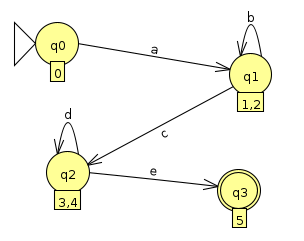
\includegraphics[width=0.5\textwidth]{p2-3.png}
\end{figure}
\end{solution}

\newpage
\section{Práctica 3}
Crear un fichero LEX, ejecutar el programa sobre él, compilar la salida y ejecutarla sobre un conjunto de datos de entrada.

\begin{solution}
	Mi fichero LEX es el siguiente:
	\lstinputlisting[backgroundcolor = \color{lightgray!35}]{p3/p3.lex}
	Básicamente clasifica las entradas en varias categorías:
	\begin{itemize}
		\item Números enteros.
		\item Números reales.
		\item DNI.
		\item NIE.
		\item Matrículas.
		\item Matrículas provinciales.
		\item Matrículas de ciclomotor.
		\item Números de Seguridad Social.
		\item Ingredientes para una tortilla de patatas.
	\end{itemize}
	Con el siguiente fichero de entrada:
	\lstinputlisting[backgroundcolor = \color{lightgray!35}]{p3/input.txt}
	se obtiene el siguiente resultado:
	\lstinputlisting[backgroundcolor = \color{lightgray!35}]{p3/output.txt}
\end{solution}
\newpage
\section{Práctica 4}
Demostrar mediante JFLAP que la siguiente gramática es ambigua:
\begin{center}
	$E \implies I$\\
	$E \implies I-E$\\
	$E \implies E-I$\\
	$I \implies a|b|c|d$
\end{center}

\begin{solution}
Tomaremos la palabra $a-b-c$ para demostrar la ambigüedad:
\begin{enumerate}
	\item Comenzamos introduciendo la gramática en JFLAP-Grammar.
	\item Accedemos a la opción \textit{Brute Force Parse}.
	\item Introducimos nuestra palabra y obtenemos su árbol de derivación:
	\begin{figure}[H]
		\centering
		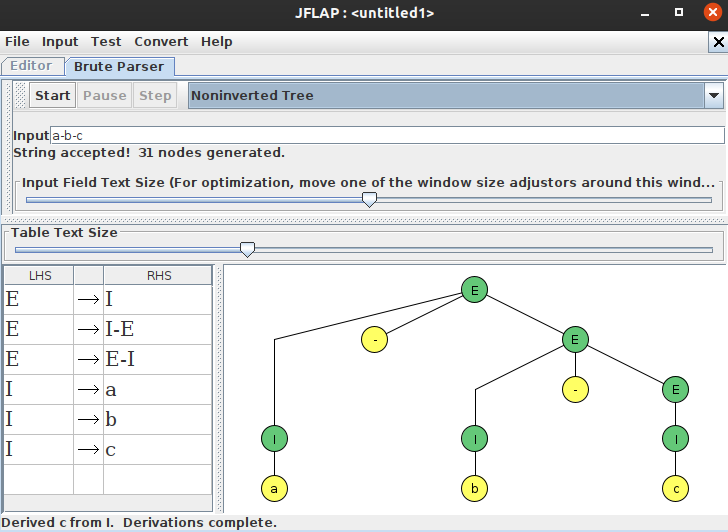
\includegraphics[width=0.75\textwidth]{p4-1.png}
	\end{figure}
	\item Ahora abrimos una nueva ventana e introducimos la gramática pero cambiando el orden de las reglas.
	\item Generamos el árbol de derivación y obtenemos lo siguiente:
	\begin{figure}[H]
		\centering
		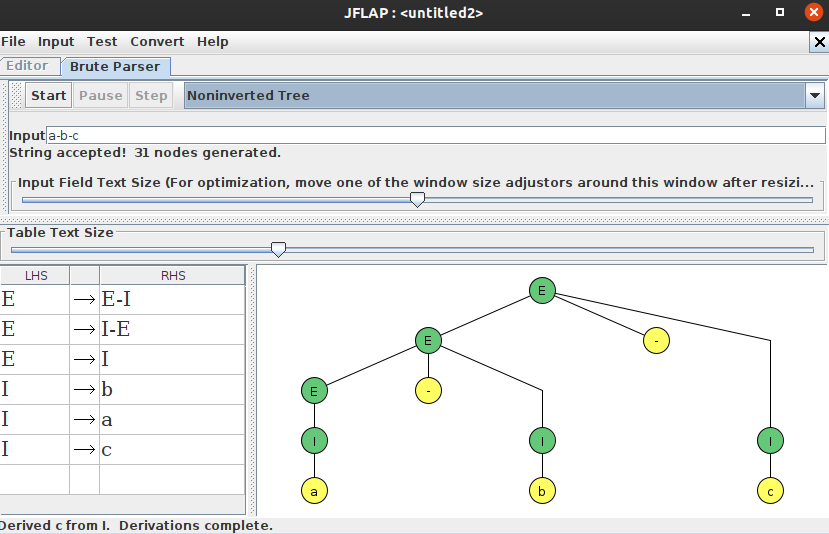
\includegraphics[width=0.75\textwidth]{p4-2.png}
	\end{figure}
	\item Vemos que los árboles son distintos para una misma palabra, por lo que concluimos que la gramática es ambigua.
\end{enumerate}


\end{solution}



\end{document}
